\documentclass[12pt,a4paper]{article}
\usepackage[utf8]{inputenc}
\usepackage[english]{babel}
\usepackage{amsmath}
\usepackage{amsfonts}
\usepackage{amssymb}
\usepackage{graphicx}
\usepackage{wrapfig}

\usepackage{color}
\usepackage{fancyvrb}

\usepackage{xspace}

\usepackage[a4paper,margin=3cm]{geometry}

\usepackage[colorlinks=true,linkcolor=black]{hyperref}

%%%%%%%%%%%%%%%%%%%%%%%%%%%%%%%%%%
%%%%%  reviewer comments  %%%%%%%%
%%%%%%%%%%%%%%%%%%%%%%%%%%%%%%%%%%
\newcommand{\comm}[2]{{\sf \(\spadesuit\){\bf #1: }{\rm \sf #2}\(\spadesuit\)}}
\newcommand{\mcomm}[2]{\marginpar{\tiny \comm{#1}{#2}}}
%\renewcommand{\comm}[2]{}
%%%%%%%%%%%%%%%%%%%%%%%%%%%%%%%%%%
\newcommand{\jbcomment}[1]{\mcomm{JB}{#1}}
\newcommand{\cocomment}[1]{\mcomm{CO}{#1}}

% Fancy code with color commands:
\DefineVerbatimEnvironment{fancycode}%
        {Verbatim}{fontsize=\footnotesize,commandchars=\\\{\}}
\DefineVerbatimEnvironment{code}%
        {Verbatim}{fontsize=\footnotesize}

%%%%%%%%%% The language %%%%%%%%%%
\newcommand{\paladim}{\textbf{Paladim}\xspace}
\newcommand{\mips}{\textsc{Mips}\xspace}
\newcommand{\mars}{Mars\xspace}


%%%%%%%%%%%%%%%%%%%%%%%%%%%%%%%%%%%%%%%%%%%%%%%%

\author{Jost Berthold, Cosmin Oancea}

\title{
\paladim \ -- Pascal And Large Array Dimensions, Introducing Main
}

\title{\vspace*{-5ex}
%      ^^^^^^^^^^^^^^ dirty hack!
    A Compiler for the \paladim Language}
\author{Group Project for the Compiler Course}

\date{Block~2, Winter 2013/14}

\begin{document}

\maketitle

\vspace*{-5ex}
\tableofcontents

\section{Introduction}

This is the description of the project for the Compilers Course
(Overs\ae{}ttere) in  block 2 of 2013-2014.
%
The project should be solved in groups of (up to) three students, and will
be evaluated as passed or failed (without a mark). You have to pass the
project task to get access to the final exam of the course.

The task is to complete the implementation of a compiler for the \paladim
language\footnote{\paladim
stands for "Pascal and large array dimensions, introducing main".},
described in detail in a later section.
The \paladim programming language is a pascal-like imperative language
with functions and procedures,
which uses multidimensional regular arrays.

\noindent
The task is \textbf{available from Tuesday, 19 Nov. 2013}.
%
A \textbf{first part} of the solution, from now on called the
\textit{\textbf{milestone}},
is \textbf{due on Friday, 6 Dec. 2013}.
%
The \textbf{final solution} must be \textbf{handed in by
Friday, 20 Dec. 2013, 2:00pm}.

\newpage

\section{The Project Task}

\subsection{Task Summary}

A partial implementation of a \paladim compiler has been prepared as a
hand-out for you.  Your task will be to add specific language features and
parts of their implementation, to produce a compiler for the full language.
Some small test programs are also provided, but you should add more of them
to test your implementation.

In brief, you need to implement the following features in the assignment:

\begin{itemize}
\setlength{\itemsep}{0.1ex}

\item A new parser for \paladim, using the tool \texttt{mosmlyac}.\\
    This subtask \emph{should be solved and described at the milestone}.

\item Integer multiplication and division, and boolean operators
(%\texttt{and},
\texttt{or}, \texttt{not});

\item Simple type inference and type checking for special functions \texttt{read} and \texttt{new};

\item code generation for indexing into arrays;

\item call-by-value-result semantics for procedure arguments.

\end{itemize}
The project tasks are described in more detail in Section~\ref{sec:tasks},
after the language description.

\subsection{Solving the Tasks and Submitting the Solution}

The project should be solved in groups of (up to) three students.
%
Solutions should be handed in by uploading code and a written 
report to the Absalon course pages.

Midway through the project, a \emph{milestone submission} should be delivered.
The milestone consists of a solution to one of the subtasks,
and a short status report on the other tasks. Its purpose is to enable early
feedback from teaching assistants about report writing style, testing
methodology, and implementation work.

The \emph{final solution} consists of the compiler code and a
project report, which describes your solutions to all subtasks
(and will thus include material submitted earlier for the milestone).
The final report will be assessed as passed or failed, without a mark.

Use the group submission function in Absalon for both
hand-ins, and indicate the names of all group members in the reports.
Approval of this task is a prerequisite for participation in the
final exam (in addition to approval of at least four of the five
weekly assignments), and \emph{cannot be resubmitted}.

\subsubsection{Important Dates}
\begin{tabbing}
\textbf{Friday, 20 Dec. 2013, 2:00pm:}~\= \kill
\textbf{Tuesday, 19 Nov. 2013:}\> The \textbf{task is available} on Absalon\\
\textbf{Friday, 6 Dec. 2013:}\>
A \textbf{milestone submission} should be handed in.\\
\textbf{Friday, 20 Dec. 2013, 2:00pm:}\>
\textbf{Final solution} must be uploaded to Absalon.\\

\end{tabbing}

\subsubsection{Milestone Submission}

The milestone submission should contain a \emph{complete solution to the first
subtask}, i.e. a parser for \paladim generated using the \emph{mosmlyac}
parser generator, including test programs. The parser should be able to parse
the new kinds of expressions introduced by task 2.
Furthermore, you should submit a written status report (2-5 pages) describing
the implementation of the parser and how you have tested it, as well as your
ideas and partial work on the other subtasks.

You should hand in two files by uploading them to Absalon:
\begin{enumerate}
\item A \texttt{zip} or \texttt{tar.gz} archive containing
    the \emph{parser grammar file} (input file for mosmlyac),
    the rest of the compiler source code (which should now use the new
    generated parser),
    and the tests you have used.
Please use the same directory structure as in the code which was handed out.

\item A written \emph{status report} describing the parser implementation, its
    integration in the compiler and how it was tested, and ideas and status
    for the other subtasks. This report may be brief (2-5 pages), but should
    contain all necessary technical information.
\end{enumerate}
Please use the group submission function in Absalon (i.e. only one submission
per group), and write the names of all group members on the title page of the
report.

\subsubsection{Final Submission}

The final solution for the project consists of
a \emph{complete implementation of all subtasks},
the \emph{test data} you have used to test them,
and a \emph{technical report} describing your implementation and tests.
%
Please upload to Absalon the following two files:
\begin{enumerate}
\item A \texttt{zip} or \texttt{tar.gz} archive containing the full implementation
	of the compiler and tests. Please use the same directory structure as
    the code which was handed out,
%    (source code in \texttt{SRC}, tests in \texttt{DATA}).
    and make sure that the provided compilation script \texttt{compile.(bat|sh)}
    works and produces your compiler as {\tt BIN/\paladim}.
\item A written \emph{report} describing and evaluating your work and the main design
	decisions you took. %in your implementation.
	The report should not exceed 16 pages of text, and must describe
	your work in sufficient technical detail (see below).

\end{enumerate}
Again,
please use the group submission function in Absalon (i.e. only one submission
per group), and write the names of all group members on the title page of the
report.
%
Your solution should demonstrate competence in the entire curriculum,
understanding of all compiler phases and the ability to thoroughly document your
solution.
%
Partial solutions will be considered if they are convincing and well-documented.

\paragraph{Writing the Report:}
The technical report about your implementations shall include justification of the changes that
were made in every compiler stage, i.e., scanner, parser, interpreter,
type checker, code generator.

You should not include the whole compiler code in the content
of your report, but you {\em must} include the parts that were either
added, i.e., new code, or substantially changed.  Add them as
Figures, or code listings in Annexes or the like.
%
If you refer to implementation code, this must also be included
in the report document.

The report shall describe how your modifications were tested, describing
how test programs were selected, and their expected behaviour and/or output.
If any of your tests do not succeed, possible reasons should be given.

Known shortcomings in type checking and compilation must be described,
and, whenever possible, you need to make suggestions on how these might
be corrected.

Your report should include all important information about your solution:
all major design decisions should be presented and justified, and all
deficiencies must be described.  Ideally, we should not need to read your
source code.
However, be concise in your description and do not include irrelevant details,
and keep the report below 16 pages.
In the end, it is largely your decision what you think is important enough
to include in the report, as long as the explicit requirements above are met.

\paragraph{Tools to Use:}
Please use the Moscow ML\footnote{Moscow ML is available at
\url{http://mosml.org}~\cite{MoscowML}, the latest version is 2.10.} compiler,
{\tt mosmlc}, to compile the code which is handed out and your modifications.
For lexical and syntactical analysis, Moscow ML's tools
{\tt mosmllex} and {\tt mosmlyac} will be used.

\noindent
To run the programs compiled by the \paladim compiler, you should use the
\mars simulator\footnote{\mars is available at
\url{http://courses.missouristate.edu/kenvollmar/mars/}~\cite{Mars}.
}.
\mars simulates a MIPS processor, and
%its usage is briefly described in the manual \texttt{mips-module.pdf}.
%It
is written in Java, so you need a Java Runtime Environment to
use it.

\noindent
We have tested our implementation and will evaluate yours with these tools.

\paragraph{Accepted Limitations:}

It is perfectly acceptable that the scanner, parser, type checker and code
generator stop at the first error encountered.
%
It can be assumed that the translated program is small, so that target
addresses for jump and branch instructions always fit into constant fields of
\mips jump instructions (i.e. label addresses fit into 16 bit, for branch
instructions).
%
It is not necessary to free memory in the heap while running the program.
You do not need to consider stack or heap overflow in your implementation.
%The actual behavior of overflow is undefined, so if errors occur during
%execution, or you see strange results, it might be due to overflow.


\section{Technical Description}


\subsection{Compiler Module Structure}

A partial implementation of the \paladim compiler has been prepared
as a starting point for your work, as well as a number of
input programs and expected output for tests.
%
This partial implementation can be found in the archive
{\it \paladim.zip}. The archive contains four subfolders:
\begin{description}
\setlength{\itemsep}{0.1ex}

\item[{\tt SRC/}:] contains the implementation of the compiler.

\item[{\tt DATA/}:] contains test inputs and expected output files.

\item[{\tt DOC/}:] contains documentation, e.g., this document and {\tt mips-module.pdf}.

\item[{\tt BIN/}:] will contain the compiler executable (binary) file.

\end{description}

To complete the task you will need to modify files in the {\tt SRC} folder,
your tests should be added to the \texttt{DATA} folder.

Files {\tt SRC/compile.sh} and {\tt SRC/compile.bat} contain commands
to rebuild all modules and the compiler under Linux and Windows, respectively.
%
The handed-out code does not generate any compiler warnings. Try to keep your
changed code free of warnings or errors as well.
%
The bundle also contains a Makefile, but you do not need to understand or
use it.


\begin{figure}[t]
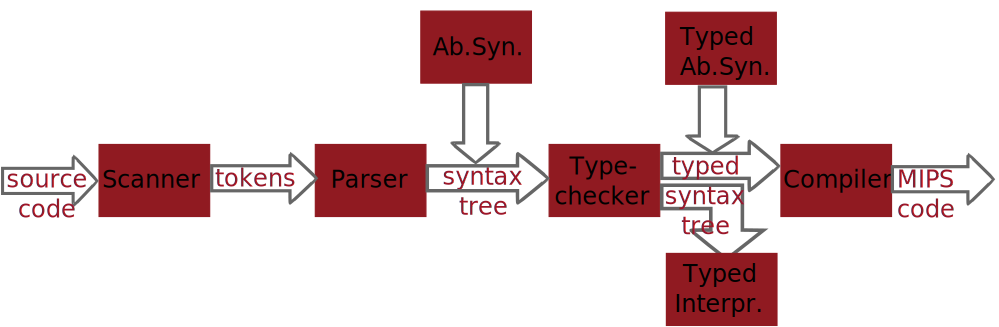
\includegraphics[width=\textwidth]{compilation}
\caption{Compiler Modules of the \paladim Compiler}
\label{fig:chain}
\end{figure}

The \paladim compiler consists of a number of modules which form a processing
chain, as depicted in Figure~\ref{fig:chain}. The following modules are part of
the compiler:

\begin{description}

\item[{\tt Lexer.lex}:] Definition of \paladim lexical tokens, used
    by \texttt{mosmllex} to generate the \paladim scanner.

\item[{\tt LL1Parser.sml}:] A top-down parser for \paladim programs,
    producing the abstract syntax tree of the input program.
    This parser will be \emph{replaced} in task 1.

\item[{\tt AbSyn.sml}:] The abstract syntax data type for \paladim programs,
       along with some helper functions to format and print entities of a
       \paladim program.

\item[{\tt Type.sml}:] Type-checker for \paladim, produces a type-checked
    abstract syntax.

\item[{\tt TpAbSyn.sml}:] The abstract syntax data type for type-checked
    \paladim programs, along with helper functions for printing and for
    retrieving type information from \paladim programs.

\item[{\tt TpInterpret.sml}:] An interpreter for type-checked \paladim
    programs (\texttt{TpAbSyn}).

\item[{\tt Compiler.sml}:] Translator from \paladim to \mips assembler.
    The translation is done directly from \paladim to \mips, i.e., without
        passing through a lower-level intermediate representation of the code.

\item[{\tt Driver.sml}:] The main program which defines the compilation chain
    (and file I/O).

\end{description}

\noindent
There are two more modules in the compiler: a register allocator
(\texttt{RegAlloc.sml}), and functions and types for \mips instructions
(\texttt{Mips.sml}). Both provide general infrastructure and are not specific
to the \paladim language implementation.
It will not be necessary to modify these files for your project.

The main program {\tt Driver.sml} is the driver of the compiler: it runs the
scanner and parser, and type-checks the program.
Depending on the given program options (\texttt{-ti} or
\texttt{-c}), it then either interprets the program, or else compiles
it to \mips code.
Processing stages after the type checker assume that the program is
type-correct and use type information in code generation and interpretation.

\subsection{The \paladim Language\label{sec:lang}}

\paladim is a Pascal-like imperative language with simple control structures
and data types.
A small example program is given here, which computes a Fibonacci number
using an array of intermediate results (dynamic programming).

\subsubsection{Lexical and Syntactic Structure}

\begin{wrapfigure}[16]{r}{0.4\textwidth}
\vspace*{-8ex}
\begin{code}[fontsize=\scriptsize, frame=lines,label=\textit{DATA/fibArray.pal}]
program fibonacciArray;

function fillFib(int n) : array of int
var r : array of int;
    i : int;
begin r    := new(n+1);
      r[0] := 0; r[1] := 1;
      i    := 1;
      while (i < n) do
         begin i  := i + 1;
               r[i] := r[i-1] + r[i-2];
         end;
      return r;
end;

procedure main()
var n : int;
    a : array of int;
begin n := read();
      if n < 1 then return;
      a := fillFib(n);
      write(a[n]); write('\n');
end; // main
\end{code}
\vspace*{-4ex}
\caption{\paladim Program to Compute Fibonacci Numbers}
\label{fig:fib}
\end{wrapfigure}

\paladim programs consist of a number of procedures and functions, the latter
returning values while the former do not. There should always be a \texttt{main}
procedure.

Functions and procedures consist of a top-level \emph{block} with
(optional) variable declarations followed by statements.
%All variables in a \paladim block are declared in the
%beginning, and
Variables can have a base type (\texttt{char, int, bool}) or an
array type (\texttt{array of ..}), which can also be nested.

The detailed syntax of \paladim is given by the grammar in Figure~\ref{fig:grammar}.
Lexical entities are characterised in the following.

\paragraph*{Identifiers} in \paladim must begin with a letter
    (ranging from $A$ to $Z$ and from $a$ to $z$),
    followed by any number of letters or digits or underscore.
   %
   Some words ({\tt if, then, function,}\ldots) are reserved keywords and
   {\em cannot} be used as identifiers.

\paragraph*{Numeric constants} are positive whole decimal numbers, formed from digits
   $0$ to $9$. Numeric constants are limited to numbers representable
   as positive integers in Moscow ML.
%
  Negative number literals are unsupported, one must write {\tt 0-1} for
  {\tt -1}).

\paragraph*{Character literals} are surrounded by single quotes
   (\texttt {'}). A character literal can be either
    a character with ASCII code between $32$ and $126$ \emph{except}
     for characters \texttt{\underline'}, \texttt {\underline"} and
     \underline{\textbackslash};
    or else, an \emph{escape sequence}, consisting of character
    \underline\textbackslash, and one of the following characters:
    \texttt{a, b, f, n, r, t, v, ?, \underline', \underline"}.
%     or
%  by an octal value between 0 and 0177, 	or by \texttt{x} and a
%  hexadecimal value between 0 and 0x7f.

\paragraph*{String literals} consist of a sequence of characters surrounded by
    double quotes (\texttt {"}). Escape sequences as described above can be used
    in string literals.

\paragraph*{Operators} are the usual arithmetic, comparison, and boolean
    binary operators.

    All binary operators are \emph{left-associative}, and have the usual
    precedence: Addition and subtraction bind
    weaker than multiplication and division, comparisons bind weaker than
    arithmetic, and boolean operators bind weaker than comparisons.

  \smallskip
\noindent
\textbf{Line comments} start by {\tt //}, and make the scanner filter out
    the rest of the line.

\noindent
\textbf{Whitespace} is irrelevant for \paladim, and no lexical atoms contain
whitespace.

\newcommand{\keyw}[1]{\mbox{\textbf{#1}}}
\newcommand{\tok}[1]{\mbox{\sc #1}}
\newcommand{\com}[1]{\mbox{\scriptsize \color{red}{#1}}}

\begin{figure}

\renewcommand{\arraystretch}{0.87}
{\scriptsize

\begin{minipage}{0.53\textwidth}
\textbf{Program structure:}\\
\fbox{
$ % $
\begin{array}{lcll}
Prog & \rightarrow & \keyw{program}\ \tok{Id}\ ;\ FunDecs \\[0.9ex]

FunDecs & \rightarrow & FunDecs \ FunDec \\
FunDecs & \rightarrow & FunDec \\[0.9ex]

FunDec & \rightarrow & \keyw{function}\ \tok{Id} ( PDecl )\ : \ Type \ Block\ ; \\
%Fun & \rightarrow & Type \ \tok{Id} \ ( ) = \ Exp  \\[0.9ex]
FunDec & \rightarrow & \keyw{procedure}\ \tok{Id} \ ( PDecl ) \ Block \ ; \\[0.9ex]

Block & \rightarrow & DBlock \ SBlock \\%[0.9ex]

DBlock & \rightarrow & \keyw{var}\ Decs \\
DBlock & \rightarrow & \varepsilon\\

SBlock & \rightarrow & \keyw{begin} \ StmtSeq \ ; \keyw{end}\\
SBlock & \rightarrow & Stmt\\%[0.9ex]

StmtSeq & \rightarrow & StmtSeq \ ; \ Stmt\\
StmtSeq & \rightarrow & Stmt

\end{array}
$ % $
}
\end{minipage}
\hfill
\begin{minipage}{0.45\textwidth}
\textbf{Variable and Parameter Declarations, Types}
\fbox{
$ % $
\begin{array}{lcll}
PDecl & \rightarrow & Params\\
PDecl & \rightarrow & \varepsilon & \com{can be empty}\\

Params & \rightarrow & Params \ ;\ Dec\\
Params & \rightarrow & Dec \\[0.9ex]

Dec & \rightarrow & \tok{Id} \ : \ Type \\[0.9ex]

Decs & \rightarrow & Decs \ Dec \ ;\\
Decs & \rightarrow & Dec  \ ; & \com{cannot be empty}\\[0.9ex]

Type & \rightarrow & \keyw{int} \\
Type & \rightarrow & \keyw{char} \\
Type & \rightarrow & \keyw{bool} \\
Type & \rightarrow & \keyw{array} \ \keyw{of} \ Type & \com{may be nested}\\
\\
\end{array}
$ % $
}
\end{minipage}

\medskip
\begin{minipage}{0.53\textwidth}
\textbf{Statements}\\
\fbox{
$ % $
\begin{array}{lcl}
Stmt & \rightarrow & \tok{Id} ( CallParams ) ~~~~~~~~~~~\com{procedure call}\\
Stmt & \rightarrow & \keyw{if}    \ Exp \ \keyw{then} \ Block\\
Stmt & \rightarrow & \keyw{if}    \ Exp \ \keyw{then} \ Block \ \keyw{else} \ Block\\
Stmt & \rightarrow & \keyw{while} \ Exp \ \keyw{do}   \ Block\\
Stmt & \rightarrow & \keyw{return}\ Ret  ~~~~~~~~~~~~~~~~~\com{maybe empty}~~~~\\
Stmt & \rightarrow & LVal \ := \ Exp ~~~~~~~~~~~~~~\com{assignment}
\end{array}
$ %$
}
\end{minipage}
\hspace*{1em}
\begin{minipage}{0.53\textwidth}
\textbf{Function and Procedure Parameters and  Index Lists}\\
\fbox{
$ % $
\begin{array}{lcll}
CallParams & \rightarrow & Exps\\
CallParams & \rightarrow & \varepsilon  & \com{may be empty}\\

Exps & \rightarrow & Exp \ , \ Exps\\
Exps & \rightarrow & Exp & \com{never empty}\\
\\[2ex]
\end{array}
$ % $
}
\end{minipage}

\medskip
\textbf{L-Values and Expressions}\\
\fbox{
$ % $
\begin{array}{lcll}
LVal & \rightarrow & \tok{Id}\\
LVal & \rightarrow & \tok{Id}[ Exps ] & \com{index into an array}\\[0.9ex]

Ret & \rightarrow & Exp & \com{return statement may or\ldots}\\
Ret & \rightarrow & \varepsilon & \com{ \ldots may not include an expression}\\[0.9ex]

Exp & \rightarrow & \tok{NumLit} \\
Exp & \rightarrow & \tok{LogicLit}\\
Exp & \rightarrow & \tok{CharLit} \\
Exp & \rightarrow & \tok{StringLit} \\
Exp & \rightarrow & \{ \ Exps\ \} & \com{Special array literal, never empty} \\
Exp & \rightarrow & LVal  & \com{simple and indexed identifiers} \\
Exp & \rightarrow & \tok{not} \ Exp & \com{boolean negation}\\
Exp & \rightarrow & Exp \ \tok{OP} \ Exp & \com{binary operations}\\
Exp & \rightarrow & ( \ Exp \  )\\
Exp & \rightarrow & \tok{ID} \ ( \ CallParams \  ) & \com{function call}\\[0.9ex]

OP & \rightarrow & \tok+ \ |\ \tok- \ |\ \tok* \ |\ \tok/ \ |\ \tok= \ |\ \tok< \ | \ \tok{and}\ | \ \tok{or}

\end{array}
$ % $
}

} % scriptsize

\renewcommand{\arraystretch}{1.0}
\caption{Syntax of \paladim}
\label{fig:grammar}
\end{figure}

\subsubsection{Meaning of \paladim Programs}
\label{sec:SpecialFuns}

\paladim is a typical typed imperative language: one can evaluate arithmetic
and boolean expressions (with the usual operations), and assign values
of appropriate type to (previously declared) variables in statements.
All \paladim expressions have a \emph{statically determined type}, and there
is \emph{no automatic conversion} between types. For example, a variable of
type \texttt{int} cannot be used as a \texttt{bool} without explicit
conversion.
Conversion between different types is realised by comparison operations and
special predefined functions (see below).

A statement for conditional execution (\texttt{if}) and a loop statement
(\texttt{while}) realise control flow in the small, while functions
(returning values) and procedures (not returning anything) provide the larger
structure of a \paladim program.

At the large scale, a \paladim program consists of a set of functions and
procedures, which may take up to nine arguments.
%
The functions and procedures used in a program may be declared in any order,
but must reside in a single file (there is no module system).
%
Every valid \paladim program must contain a procedure called \texttt{main};
a \paladim program is executed by invoking it. % this \texttt{main} procedure.

\bigskip
\paladim provides some \textbf{predefined functions} for special tasks:
\begin{description}
\item[\tt chr] takes an integer argument and (returns) converts it to
        a char value, e.g., \texttt{chr(97)} returns character \texttt{'a'}.
\item[\tt ord] takes an character argument and (returns) converts it to an
        integer value, e.g., \texttt{ord('a')} returns integer \texttt{97}.
\item[\tt read] is a function without parameters which reads a value of basic type
                    \texttt{int}, \texttt{bool} or \texttt{char}
                    from the console and returns it. The
                    (basic) type of the result is determined by the type checker
                    from the context in which \texttt{read} is used
                    (read is \emph{polymorphic}).
    Booleans are read/written as \texttt{int} values (0 is \emph{false}, 1 is \emph{true}).

\item[\tt write] is a polymorphic procedure which takes exactly one
    argument, and prints out the value of the argument on the console.
    For the moment, \texttt{write} supports arguments of
        basic type (int, char, or bool).

\item[\tt new,len] are special arrays functions described in the
following section. %~\ref{sec:arraylayout}.

\end{description}


\subsubsection{Arrays in \paladim}
\label{sec:arraylayout}

Variables in a \paladim program may be declared to have array type, where
the arrays can also be nested.
For example, identifier \texttt{a} can be declared to hold a $3$-dimensional
array of \texttt{int}s, by declaration \texttt{a~:~array~of~array~of~array~of~int}.
The number of dimensions of an array is called the {\em rank},
e.g., the rank of \texttt{a} is $3$.

The special function {\tt new} allocates a new array.
The statement \texttt{a := new(3,4,5)}
will allocate a new array with $3\cdot 4 \cdot 5 = 60$ integer elements, where
all elements are initialized to zero, and assign it to a variable \texttt{a}.
%The size of a {\tt bool} and {\tt char} element is $1$ byte.
A runtime error is raised if any of the arguments (sizes for each array
dimension) is less or equal to zero.

\begin{figure}[h]%[tbh]
\includegraphics[scale=0.37]{Figures/ArrayLayout}
%\includefigure[scale=1.5]{Figures/Arrays}
\hrule
\vspace*{-1ex}
\caption{Array Layout.}
\label{fig:ArrLayout} %
\vspace*{-1ex}
\end{figure}

The left-hand side of Figure~\ref{fig:ArrLayout} shows the array layout of
the created array (in the \paladim heap): The header of an $n$-dimensional
array consists of $2\cdot n$ words (one word is $4$ bytes):
The first $n$, generically denoted by $d_1, \ldots, d_n$ store the size in
each dimension, in our case \texttt{3}, \texttt{4}, and \texttt{5}.
The next $n-1$ words, denoted by $s_1,\ldots, s_{n-1}$ are the strides\footnote{
The stride of dimension $i$ can be intuitively described as
the number of elements which are jumped in a row-major array layout when
increasing only the $i^{th}$ index by one.}
of the first $n-1$ dimensions. They are computed recursively from the last
dimension:
$s_{n} = 1$, $s_i = s_{i+1} \cdot d_{i+1}$.   In our example, $s_3 = 1$
(not represented), $s_2 = 1\cdot 5 = 5$ and $s_1 = 4\cdot 5 = 20$.
Finally, the last word of the array is a pointer to the array's 
\emph{data area} in memory. %, a ($1$-d) memory area
%which holds the array \emph{data}.
%
The size of this data area is $d_1 \cdot d_2 \cdot \ldots d_n \cdot s$
bytes, where
$s$ is the size of the array base type ($4$ Bytes for \texttt{int},
$1$ Byte for \texttt{bool} and \texttt{char}).\footnote{For a char or bool
array, the allocated area is rounded up to the next multiple of $4$, to
preserve alignment.}
The size in the example
$3 \cdot 4 \cdot 5 \cdot 4 = 240$ Bytes (60 \texttt{int} elements).

Subsequently, one can assign a new value to an element of \texttt{a} via an
\emph{indexed LValue} assignment, e.g., \texttt{a[1,0,2] := 3}, and
also read and use a value inside \texttt{a} via indexing, e.g.,
\texttt{write(a[1,0,2])}.
The address computation for indexing into an existing array is illustrated
on the right of Figure~\ref{fig:ArrLayout}.
The flat index of the respective indexed element inside the array's data area
is computed by summing up the products of index and stride in each dimension,
i.e., $i_1\cdot s_1 + \ldots + i_n \cdot s_n$
(where $s_n$ is always $1$).
In our example, the index \texttt{a[1,0,2]} corresponds to an offset of
$ 1 \cdot 20 + 0 \cdot 5 + 2 \cdot 1 = 22$ from the start of the array,
hence the $22^{nd}$ element in the array's content is set to $3$.
If any given index is negative or greater than the corresponding dimension
size (e.g. if for {\texttt{a[i$_1$,\ldots,i$_n$]}, there is a $i_k > d_k-1$
or $i_k < 0$), execution stops with a runtime error.

The \emph{size in one dimension} of an array can be queried at runtime by
the special function {\tt len}. In our example, {\tt len(0,a)} would
return $3$, the size in the first dimension. Similarly, {\tt len(1,a)}
and {\tt len(2,a)} would return $4$ and $5$. If the first argument
of {\tt len} is negative or greater than the rank of the array, a runtime
error is raised (for instance,
both {\tt len(-1,a)} and {\tt len(4,a)} result in runtime errors).

%\medskip
Note that both {\tt new} and {\tt len} are polymorphic function:
%\begin{itemize}
%\setlength{\itemsep}{-1ex}
%\item[\tt new]
\texttt{new} receives an \emph{arbitrary number} \texttt{n} of
    integer-type arguments, and the type checker must determine the
    \emph{type of the result array} from the context where \texttt{new}
    is used.
%\item[\tt len]
\texttt{len} takes two arguments: an integer value and an array
        \emph{of arbitrary type}, and returns an integer, i.e., the size
        of the \texttt{n$^{th}$} dimension of array \texttt{a}.
%\end{itemize}

\subsection{Project Tasks}
\label{sec:tasks}

\subsubsection*
  {1. A Parser for \paladim Using the \emph{mosmlyac} Parser Generator}

The handed-out code comes with a top-down parser for \paladim. This parser
does not support some of the necessary syntax for subtask 2, and it is
hard to maintain.

Your task is to replace this parser by one which is generated using the
\emph{mosmlyac} parser generator, and which supports all necessary syntax
for the other tasks.
This parser's \texttt{Parser.grm} file should be written from scratch.

Note that you must change \texttt{Driver.sml} to use \emph{your} implementation
instead of the top-down parser. This is done by uncommenting the appropriate
lines in the body of the \texttt{compile} function.\\[1ex]
\textbf{The solution to this subtask should be delivered with the milestone.}

\subsubsection*
  {2. Integer Multiplication and Division, and Boolean Operators}

The delivered compiler only implements addition and subtraction.
Your task is to implement full support for arithmetic operations, i.e.
multiplication and division (which have precedence over addition and
subtraction).

Furthermore, the compiler only implements the boolean \texttt{and} operator.
You should implement support for the missing boolean operators,
i.e. \texttt{or} and \texttt{not}. Conjunction (\texttt{and}) has precedence
over disjunction (\texttt{or}), but binds weaker than the unary negation
(\texttt{not}).
As an example, the expression
%\hspace*{4em}
$ b\ =\ c \ \keyw{or}\ \keyw{not} \ a\ =\ b\ \keyw{and}\ a\ =\ c$% \\
should be parsed as %\\
%\hspace*{4em}
$ (b=c)\ \keyw{or}\ ((\keyw{not} \ (a = b))\ \keyw{and}\ (a =c))$.
\\[1ex]
\textbf{The parser of your milestone submission should be able to parse
expressions with these operators correctly.}

\subsubsection*{3. Simple Type Inference and Type Checking the \texttt{new} Function}

The special functions \texttt{read} and \texttt{new} require the type checker
to determine their particular type from the calling context. This task is
about enabling this inference, requiring you to modify the function
\texttt{typeCheckExp} in file \texttt{Type.sml}.
%and consists of two parts:\\

To type-check calls to \texttt{read}, type-checking for expressions must,
whenever possible, determine an \emph{expected type} from the context of the
expression, and pass this expected type down as an inherited attribute when
type-checking any sub-expressions).
%
For example, if a plus-expression is type-checked, its two %constituent
subexpressions are expected to be \texttt{int}s. The inherited attribute
allows for type-checking expressions like \texttt{read() + read()}
because the context determines that both \texttt{read()} should return
\texttt{int} values.
%
Similarly, one can type-check \texttt{chr(read()) = read()}
because the context determines that
%\vspace{-1ex}
%\begin{itemize}
%    \item
(a) the first \texttt{read} should return an \texttt{int},
            since function \texttt{chr} takes an \texttt{int} argument,
%\vspace{-1ex}
%\item
and (b) the second \texttt{read} should return a \texttt{char}, since 
            the arguments of a 
            comparison must have the same type, and \texttt{chr}
            returns \texttt{char}.

%\end{itemize} \vspace{-1ex}

For simplicity, it is allowed that \texttt{read() = chr(read())}
fails to type-check, i.e. it is fine to use (only) the resulting type
of the \emph{left} sub-expression as an expected type for the \emph{right} sub-expression,
rather than implementing all possible cases.
Finally, an expression like \texttt{read() = read()}
will fail to type-check because there is no unique way of determining
the return type of the two \texttt{read()}, e.g., they may both return
a boolean value, or a character value, or an integer value.

As a second, related task, you should implement type-checking for the
predefined (polymorphic) function \texttt{new},
which was explained in Section~\ref{sec:arraylayout}.
%
Function \texttt{new} requires checking that all arguments are of
integer type, and the expected type attribute is needed to determine
the type of the resulting array (and especially the element size to allocate).
%Function \texttt{len} requires checking that the first argument
%is an integer and the second is an array.

{\bf See Appendix~\ref{sec:task3hints} for more hints.}

%Function \texttt{new} is polymorphic in that it may create arrays
%of all three basic types and arbitrary number of dimensions, hence
%type checking a call to \texttt{new} uses its expected type
%(inherited) attribute.   Function \texttt{len} is polymorphic
%in that it can receive as second argument any type of array
%(but the first argument should be an int).

%\texttt{len(n, a)} returns the size of the \texttt{n$^{th}$} dimension
%of array \texttt{a}, and \texttt{new(n$_1$,..,n$_k$)}
%and  which were described

%The handed-out compiler does not provide the described \texttt{read} and
%\texttt{write} functions, but only specialised versions \texttt{readInt},
%\texttt{readChar}, \texttt{writeInt}, and \texttt{writeChar}.
%
%Your task is to implement a type inference (in the type checker) which finds
%the type of output and uses the correct \texttt{write} function for that type.
%A related, but more difficult, problem is to find the type of input
%obtained from the user by a \texttt{read} call.
%
%\comm{JB}{need to give hints for this one, especially the tricky
%\texttt{read} inference.}
%
%To see why this is more difficult, consider a program which contains the
%following statement:
%\begin{code}
%if read() + 1 < read() then write("smaller!")
%\end{code}
%Your implementation will have to use an inherited attribute which provides
%an expected type for \texttt{read}.
%\comm{JB}{This attribute is already prepared in the type-checking code, but not used anywhere so far. (?)}
%

\subsubsection*{4. Type Checking and Code Generation for Array Indexing}

As described in Section~\ref{sec:arraylayout},
a variable holding an array can be used in indexing expressions, both to use
the stored value in an expression, and to assign a new value to the location in
an assignment.
%
%The implementation of these indexed L-values must compute the memory address of
%the corresponding array element, in order to access (read or write) the memory
%area where those values are stored.
%
This array indexing is not implemented in the type checker and in the compiler,
your task is to implement it.

%\begin{itemize} \vspace{-1ex}
%    \item 
Type-check an indexed array by adding the corresponding
            case to the function \texttt{typeCheckExp} in file \texttt{Type.sml}.
            You must check that all indices are integers,
            and that the number of indices matches the array's rank, i.e., full indexing.
%            \vspace{-1ex}

%    \item 
Generate machine code to compute the address of a certain array
            element by adding the corresponding case to function \texttt{compileLVal}
            in file \texttt{Compiler.sml}.
%
            You should review the array layout description
            in Section~\ref{sec:arraylayout} to find out how the respective address
            offset is computed, involving the stored \emph{strides} (and the
            type information about the array elements).
            Your implementation should raise a runtime error when an index
            is out of bounds in any of the dimensions.

%    \item[BONUS:] 
\textbf{Bonus:} The computation of the flat index into the array's content can be
            accomplished in a manner of similar efficiency to the one described
            in Section~\ref{sec:arraylayout}, but which uses only the array's
            dimension sizes (and {\em not} its strides).   A bonus will be offered
            if you present how this may be accomplished and/or if you actually
            implement it (instead of the suggested solution).
%            For example, denoting by \texttt{\{s$_1$,..,s$_{n-1}$, 1\}}
%            the strides of the n-dimensional array \texttt{a}, the offset from the start
%            address of the content of the array for \texttt{a[i$_1$,..,i$_n$]} is \\
%            $(i_1 \times s_1 + \ldots + i_{n-1} \times s_{n-1} + i_n) \times \mbox{\tt sizeof}(btp)$\\
%            where $btp$ denotes the size of the array's basic type ($4$ for int and $1$ for bool/char).
%            \vspace{-1ex}
%\end{itemize}

{\bf See Appendix~\ref{sec:task4hints} for more hints.}

\subsubsection*{5. Call-by-Value-Result Semantics for Procedures}

In many languages, procedures are used when it is necessary to return
more than one value from a subroutine.
Procedure calls in the \paladim language should therefore copy back their
argument values, in a \emph{call-by-value-result} policy.

\begin{wrapfigure}[11]{r}{0.4\textwidth}
\vspace*{-4ex}
\begin{code}[frame=lines,fontsize=\scriptsize,label=\textit{DATA/proctest.pal}]
program proctest;
procedure f(a : int; b : int)
begin a := a + 1; b := b + 1; end;

procedure main()
var x : int; y : int;
begin
   x := 2; y := 3;
   f(x, y);
   write(x); write(' '); write(y);
end;
\end{code}
\vspace*{-4ex}
\caption{\paladim example program using call-by-value-result}
\label{fig:proctest}
\end{wrapfigure}

For example, the program in Figure~\ref{fig:proctest} should output \texttt{3 4}, i.e.,
\texttt{x} and \texttt{y} are \emph{copied in} to \texttt{a} and \texttt{b} at
the beginning of the call to \texttt{f}, and upon return from \texttt{f}, the
values of \texttt{a} and \texttt{b} are \emph{copied out} into \texttt{x} and
\texttt{y}, respectively.

Your task is to implement a \emph{call-by-value-result} policy for \paladim
procedures in the interpreter and in the \mips code generator, by modifying
the \texttt{callFun} function in 
\texttt{TpInterpret.sml} and functions \texttt{compileF} and
\texttt{compileStmt} (case for procedure call) in \texttt{Compile.sml}.

\smallskip
\textbf{Interpreter Hint}:
Remember that each function/procedure call maintains its own symbol table 
that associates a variable name with its value. 
For any actual-argument expression that is a variable, you need to 
(i) get the final value, i.e., after the call, of the corresponding formal 
argument of the procedure, and 
(ii) to update the corresponding entry in the symbol table of the caller procedure.

%In the interpreter, you need to keep in mind that procedures and the code
%that calls procedures use different variable tables, and that your job is to
%move some resulting values from the procedures' tables to the caller's table.

\smallskip
\textbf{Code-Generator Hint}: 
In the compiler, code already exists that moves actual arguments, stored in 
symbolic registers, to named (caller) registers when calling procedures and functions.  
The code generated for a procedure needs to be modified to move the symbolic 
registers associated to the formal arguments back into their corresponding 
named (caller) registers at the very end of the function execution. 
The code generated for a procedure
{\em call} need to be modified so that immediately after the call, the
symbolic registers holding the actual arguments are updated with the
values of their corresponding (named) caller registers.

%Hint: In the compiler, code already exists that moves variables to callee registers
%when calling procedures and functions. For procedures, you need to move those
%variables back into the registers when the procedure is finished.



%%%%%%%%%%%%%%%%%%%%%%%%%%%%%%%%%%%%%%%%%%%%%%%%%
\newpage
\appendix

\nocite{PattersonHennessy}
\nocite{Torben2011}
%\nocite{TorbenDIKU}
\nocite{MipsModule}

\bibliographystyle{unsrt}
\renewcommand{\refname}{\section{Reading Material}}

\bibliography{CB13}
%\bibliography{GroupProj}



\section{Type Checking Hints for Tasks $2$, $3$ and $5$}
\label{sec:task3hints}

\paladim is a strongly (statically) typed language, i.e., each expression,
function, etc., has a unique type that is computed at compile time.
The type checking phase, implemented in file {\tt Type.sml} via 
{\tt typeCheck*} functions, receives as input an untyped program, i.e., 
that uses the representation of file {\tt AbSyn.sml}, and verifies 
that all type rules are satisfied and produces a typed program, 
i.e., that uses the representation of file {\tt TpAbSyn.sml}.

The untyped representation, i.e., {\tt AbSyn.sml}, targets ease of 
parsing, e.g., the array type is defined recursively as  
{\tt datatype Type = ... | Array Type * Pos}, and provides
very limited type support.

The typed representation, i.e., {\tt TpAbSyn.sml}, is more suited 
for implementing code transformations such as code generation.
For example the array type is defined as
{\tt Array of int * BasicType}, where the first parameter is the
array's rank and {\tt BasicType} is one of {\tt Int}, {\tt Char} 
or {\tt Bool}.   
%
More importantly, the typed representation retains whatever
(type) information is necessary to easily compute the type
of values, expressions, statements and function by means of 
{\tt typeOfVal}, {\tt typeOfExp}, {\tt typeOfStmt}, 
and {\tt typeOfFun} functions, respectively.
%
For example, the representation of a variable identifier contains its type,
i.e., {\tt type Ident = string * Type}, and the representation of a function 
identifier contains the function signature,
i.e., {\tt type FIdent = string * (Type list * Type option)}, 
where the list of types corresponds to the arguments' types and
the type option corresponds to the return type of a function 
(and is {\tt NONE} for procedures).


%Type checking is done by traversing the abstract syntax tree while propagating
%type constraints to each node's subcomponents when necessary. If the type
%checker at any point in the traversal finds that a constraint is violated, the
%type checker will stop and throw an exception. Otherwise, a new abstract
%syntax tree is returned where all types for functions, statements, blocks and
%expressions are determined.

%The actual traversal happens in \texttt{Type.sml} with the \texttt{typeCheck*}
%functions. Let's focus on \texttt{typeCheckExp} to get an idea how it works.

Tasks $2$, $3$, and $4$ requires implementing parts of function {\tt typeCheckExp},
whose signature is presented below.
 
\vspace{-1ex}
\vbox{ \begin{Verbatim}
typeCheckExp ( vtab: VTab, f: AbSyn.Exp, etp: ExpectType ): TpAbSyn.Exp

Type checks an expression:
  Input : 1. the vtable, which associates a variable with its type
          2. an untyped expression, i.e., `AbSyn.Exp',
          3. an expected type,derived from the context (inherited atrib)

  Output: a typed expression, i.e. `TpAbSyn.Exp'.

\end{Verbatim}
}\vspace{-1ex}

Note that \texttt{typeCheckExp} returns an expression, and thus we are able to
use \texttt{typeOfExp} if we need the types of the subexpressions. (hint: have
a look at the pattern matching case in \texttt{typeCheckExp} for \texttt{Plus}.)

The expected type of the expression, {\tt etp}, is used for type checking
polymorphic expressions, such as calls to {\tt read()}, which cannot be 
uniquely typed otherwise. If {\tt etp} is unknown at such points then 
type checking fails by throwing an exception, e.g., see the pattern matching 
case in \texttt{typeCheckExp} for \texttt{AbSyn.FunApp ("read"...)}.

%Also note that \texttt{etp} is the expected type of the expression, and thus an
%exception should be thrown if the constraint is violated. (hint: have a look at
%the pattern matching case in \texttt{typeCheckExp} for \texttt{AbSyn.FunApp ("read"...)}.)

The datatype of \texttt{etp} is \texttt{ExpectType} which is also located in
\texttt{Type.sml} and looks like this:

\vspace{-1ex}
\vbox{ \begin{Verbatim}
datatype ExpectType = SomeArray of TpAbSyn.BasicType
                    | KnownType of TpAbSyn.Type
                    | UnknownType
\end{Verbatim}
}\vspace{-1ex}
Constructor \texttt{KnownType} is used when the expected type is fully known
(while \texttt{SomeArray} should be used when only the basic type of an array 
 is known, but not the array's rank).  

Non-trivial examples of how the expected type is computed/propagated are, 
for example, (i) the type checking of a function call, in which the expected 
types of the actual arguments are determined from the function's signature, 
see implementation of {\tt typeCheckExp( vtab, AbSyn.FunApp (fid, args, pos), \_)}, or
(ii) the type checking of assignment statements, in which the expected type
of the right-hand-side expression is determined from the type of the 
left-hand side variable, see {\tt typeCheckStmt( vtab, AbSyn.Assign(AbSyn.Var(id), e, pos) )}.


\section{Code Generation Hints for Task 4}
\label{sec:task4hints}

Code generation is implemented in file \texttt{Compiler.sml} by a set of
mutual recursive functions ({\tt compile*}) that correspond to the 
constructs of the abstract syntax tree.
For example, generating code for a function ({\tt compileF}) requires
generating code for all statements in the function body ({\tt compileStmt}),
which requires generating code for the statement's expressions ({\tt compileExp}), etc.

Task $4$ requires you to implement the following case of function \texttt{compileLVal}:
\vspace{-1ex}
\begin{verbatim}
compileLVal ( vtab : VTab, Index((n,t),inds) : LVAL, pos : Pos ) : 
            ( Mips.mips list * Location )
\end{verbatim}
where detailed comments are provided at that point in file {\tt Compile.sml}.\\
%
The arguments of {\tt compileLVal} are:
\begin{description}
    \item[\texttt{vtab}] A symbol table that maps any variable name to a register name,
                            i.e., the register that will record the variable's value.
    \item[\texttt{Index ((n,t),inds)}]\hfill \\
        The index which needs to be compiled, where \texttt{n} is the name
        of the array, \texttt{t} is the type of array-variable {\tt n}, and
        \texttt{inds} is the list of integer-expression indices.
    \item[\texttt{pos}] 
        The position of the {\tt LVal} in the source code, for use in error messages.
\end{description}

Function {\tt compileLVal} returns a list of {\sc mips} instructions, 
i.e., {\tt Mips.mips list}, that computes the (memory address) location of 
the indexed element, and the name of the register that records this location
({\tt Location}).

A location is represented via one of the two constructors below:
\begin{verbatim}
  datatype Location = Reg of string (* in given register *)
                    | Mem of string (* at memory address held in register *)

\end{verbatim}
in order to distinguish between registers holding a value and registers 
holding a memory address.   More precisely, when compiling an l-value
that corresponds to a variable we use constructor {\tt Reg}, and
when compiling an array index we use constructor {\tt Mem}.
For code examples that illustrate how {\tt Location} is used, please 
take a look at the implementation of an assignment statement in \texttt{compileStmt}.
%In order to accommodate that an \texttt{LVal} can be either a variable or an
%index into an array in memory, a custom datatype has been created:
%
%The location datatype is thus used to distinguished between values and
%pointers. Variables are loaded directly into registers, while indexed
%variables are represented as pointers to the indexed element in the array. For
%examples on how their usage differ you should look at the {\it Assign} case in
%\texttt{compileStmt}.

%\part*{Appendix}
%\addcontentsline{toc}{part}{Appendix: Description of the \paladim Compiler Modules}
%\section*{Description of the \paladim Compiler Modules}
%\label{sec:modules}


\end{document}
